\documentclass{scrbook}
\KOMAoptions{
	DIV=12,
	fontsize=12pt,
	paper=letter,
	twoside=false,
	parskip=half-,
}
\usepackage[onehalfspacing, nodisplayskipstretch]{setspace}
\usepackage{amsmath, amssymb, amsfonts}
\usepackage{enumitem}

\usepackage{tikz}
\usetikzlibrary{arrows}
\usepackage{subcaption}

\usepackage[american]{babel}
\usepackage{csquotes}
\usepackage[en-US]{datetime2}
\DTMlangsetup[en-US]{showdayofmonth=false}

\usepackage{amsthm}
\newtheorem{theorem}{Theorem}
\newtheorem{lemma}[theorem]{Lemma}
\newtheorem{proposition}[theorem]{Proposition}
\newtheorem{corollary}[theorem]{Corollary}
\theoremstyle{definition}
\newtheorem{problem}{Problem}
\newtheorem{question}{Question}
\newtheorem{definition}[theorem]{Definition}
\newtheorem{example}[theorem]{Example}

\newcommand{\vocab}[1]{\textbf{#1}}

\usepackage[dvipsnames, rgb]{xcolor}
\usepackage{mathtools}
\renewcommand{\geq}{\geqslant}
\renewcommand{\ge}{\geqslant}
\renewcommand{\leq}{\leqslant}
\renewcommand{\le}{\leqslant}
\usepackage{booktabs}
\usepackage{ytableau}
\ytableausetup{centertableaux, smalltableaux}

\DeclareMathOperator\Par{\mathsf{Par}}
\DeclareMathOperator\Sym{\mathsf{Sym}}
\DeclareMathOperator\sym{\mathcal{S}}
\DeclareMathOperator\cyc{\mathsf{cyc}}
\DeclareMathOperator\inv{\mathsf{inv}}
\DeclareMathOperator\sign{\mathsf{sign}}
\DeclareMathOperator\Grassmanian{\mathsf{Gr}}
\DeclareMathOperator\GL{\mathsf{Gr}}
\DeclareMathOperator\id{\mathsf{id}}
\DeclareMathOperator\Aut{\mathsf{Aut}}
\DeclareMathOperator\Mat{\mathcal{M}}
\newcommand{\qbinom}[3][q]{\genfrac{[}{]}{0pt}{}{#2}{#3}_{#1}}
\newcommand{\integers}{\mathbb{Z}}
\newcommand{\nonnegatives}{\mathbb{N}}
\newcommand{\positives}{\integers_{> 0}}
\newcommand{\rationals}{\mathbb{Q}}
\newcommand{\reals}{\mathbb{R}}
\newcommand{\complexes}{\mathbb{C}}

\newcommand\interval[1]{
  \if#11
    \{1\}
  \else
    \if#12
      \{1, 2\}
    \else
      \if#13
        \{1, 2, 3\}
      \else
        \if#14
          \{1, 2, 3, 4\}
        \else
          \left\{1, \dots, #1\right\}
        \fi
      \fi
    \fi
  \fi
}

\newcommand\sg[1]{\EuScript{S}_{#1}}
\newcommand\eltr[1]{
    \sigma_{#1}
}

\usepackage{listofitems}

\newcommand\perm[2][,]{%
  \readlist\thecycle{#2}%
    [\foreachitem\i\in\thecycle{\ifnum\icnt=1\else#1\fi\i}]%
}
\newcommand\tuple[2][]{%
  \readlist\thecycle{#2}%
  \foreachitem\i\in\thecycle{\ifnum\icnt=1\else#1\fi\i}%
}
\newcommand\word[2][]{%
  \def\temp{#2}\ifx\temp\empty%
    \varnothing%
  \else%
    \readlist\thecycle{#2}%
      \foreachitem\i\in\thecycle{\ifnum\icnt=1\else#1\fi\i}%
  \fi%
}
\newcommand\composition[2][]{%
  \def\temp{#2}\ifx\temp\empty%
    \varnothing%
  \else%
    \readlist\thecycle{#2}%
      \foreachitem\i\in\thecycle{\ifnum\icnt=1\else#1\fi\i}%
  \fi%
}


% https://tex.stackexchange.com/questions/343136/inline-spacing-within-the-cases-command-when-document-is-in-doublespace-mode
\makeatletter
\newcommand\new@setfontsize[3]{%
    \ifx \protect \@typeset@protect \let \@currsize #1\fi \fontsize {#2}{#3}\selectfont
}
\let\orig@setfontsize\@setfontsize
\let\orig@cases\cases
\let\endorig@cases\endcases

\renewenvironment{cases}{%
    \let\@setfontsize\new@setfontsize
    \setstretch{\setspace@singlespace}%
    \let\setfontsize\orig@setfontsize
    \orig@cases
}{%
    \endorig@cases
}
\makeatother

\usepackage[style=alphabetic, backend=biber,isbn=false,url=false]{biblatex} 
\addbibresource{references.bib}

\title{Notes for Symmetric Functions}
\author{Guilherme Zeus Dantas e Moura}

\begin{document}
	\maketitle

    %\chapter{Motivation}

\section{Modern motivation}

People study symmetric functions because they want to:
\begin{itemize}
    \item understand symmetric groups;
    \item understand general linear groups;
    \item do combinatorics and don't care about the rest;
    \item do algebraic geometry.
\end{itemize}

\section{Historical motivation}

Before representation theory, people were interested in question like the following:

\begin{question}
    Let the special linear group \(\operatorname{SL}_n\) acting on the matrix space \(\mathcal{M}_{n \times m}\).
    Also let the special linear group \(\operatorname{SL}_n\) act on the polynomial space in variables \(x_{ij}\) by
    \begin{equation*}
        A \cdot p(v) = p(A^{-1}v).
    \end{equation*}
    Which polynomials are invariant under such linear change of coordinates?
\end{question}

Constant polynomials are invariant, but what else?
By the defining property of the special linear group that the determinant of its elements is 1,
the determinant polynomials of the \(\binom{M}{n}\) submatrices are invariant.
These polynomials are the generators of the algebra of invariants of the special linear group acting on the polynomial space.
This fact is known as \vocab{Hilbert's fundamental theorem of invariant theory}.

Some things are nice about this algebra.
For example, the invariantes are finitely generated by these \(\binom{m}{n}\) polynomials.
The relations between these generators are also known,
and are called \vocab{Plücker relations}.

People were excited about this that they wanted to generalize this to other groups.
In general, let \(G\) be a group acting on a finite-dimensional vector space \(V\) over \(\mathbb{C}\), and let \(\pi \colon G \mapsto \operatorname{GL}(V)\) be a group homomorphism.
Then, we get an action on \(\mathbb{C}[V]\), the space of polynomials functions on \(V\),%
\footnote{To be more concrete, choose a basis for \(V\) and write a polynomial as a polynomial in the coordinates of the basis.}
by 
\begin{equation*}
    g \cdot p(v) = p(\pi(g)^{-1}v).
\end{equation*}
We get invariants \(\mathbb{C}[V]^G\), the space of polynomials invariant under the action of \(G\).
People did all sorts of examples for \(V\)'s and \(G\)'s.

What kinds of questions can we ask?

\begin{question}
    Is \(\mathbb{C}[V]^G\) finitely generated?
\end{question}

For most of the examples, the answer is yes.

\begin{question}
    If so, what are the minimal generators and what are the relations between them?
\end{question}

People did it all over the place and found relations similar to the Plücker relations.

We will spend the term studying the best success story of this program,
and all of other examples will be trying to mimic this success story.

For us, the group will be the symmetric group \(G = S_n\) acting on the vector space \(V = \mathbb{C}^n\), with \(G\) acting as the permutation matrices.
Then, \(\mathbb{C}[V]^G = \Sym_n\) is our main object of study, the space of symmetric functions.%
\footnote{Fun fact: the symmetric group is named ``symmetric'' after the symmetric functions.}

We'll see that it has the best possible properties that we could hope for.
It is finitely generated by \(n\) elements, and they have no relations between them.
We can talk about basis of \(\Sym_n\).

Also, \(\Sym_n\) is basically a representation ring of the general linear group \(\operatorname{GL}_n\).
It is also basically a representation ring of the symmetric group \(S_n\).
It is also basically the cohomology ring of the Grassmannian.

It also solves other problems, like
\begin{question}[Horn problem]
    If \(A\), \(B\), \(C\) are Hermitean matrices
    with \(A + B = C\),
    how do the eigenvalues of \(C\) depend on the eigenvalues of \(A\) and \(B\)?
\end{question}
    \chapter{Formal Power Series}

In this chapter, we introduce formal power series.

To remove possible ambiguities,
note that
rings are assumed to have a multiplicative identity,
rings are not necessarily commutative, and
the multiplicative identity of a subring is the same as the multiplicative identity of the parent ring.

Let \(R\) be a ring.
As a set, let \(R[[x]]\) be \(R^{\nonnegatives}\), the set of all infinite sequences of elements of \(R\) indexed by the nonnegative integers.
In other words, \(R[[x]]\) is the set of all sequences \((a_n)_{n=0}^\infty\) where each \(a_n \in R\).

Given two sequences \((a_n)_{n=0}^\infty\) and \((b_n)_{n=0}^\infty\) in \(R[[x]]\), we define their sum as
\begin{equation}
    (a_n)_{n=0}^\infty + (b_n)_{n=0}^\infty = (a_n + b_n)_{n=0}^\infty
\end{equation}
and their product as
\begin{equation}
    (a_n)_{n=0}^\infty \cdot (b_n)_{n=0}^\infty = \left( \sum_{j=0}^n a_j b_{n-j} \right)_{n=0}^\infty.
\end{equation}
Such product is known as the \vocab{Cauchy product} of the two sequences.
With these operations, \(R[[x]]\) is a ring with additive identity \((0, 0, 0, \dots)\) and multiplicative identity \((1, 0, 0, \dots)\).

The ring \(R\) is embedded in \(R[[x]]\) via the map \(r \mapsto (r, 0, 0, \dots)\).
This allows us to view \(R\) as a subring of \(R[[x]]\).
Moreover, the polynomial ring \(R[x]\) is embedded in \(R[[x]]\) via the map \(r_0 + r_1 x + \cdots + r_n x^n \mapsto (r_0, r_1, \dots, r_n, 0, 0, \dots)\).
This allows us to view \(R[x]\) as a subring of \(R[[x]]\).

The embedding of \(R[x]\) into \(R[[x]]\) motivates the use of a similar notation for elements of \(R[[x]]\).
We designate the sequence \(A = (a_n)_{n=0}^\infty\) by the formal expression
\begin{equation*}
    A(x) = \sum_{n=0}^\infty a_n x^n,
\end{equation*}
even though such expression is not formed by the operation of addition in \(R[[x]]\).
We write \([x^k]A(x)\) to denote \(a_k\).

This notational convention allows for convenient reformuations of the definitions of addition and multiplication in \(R[[x]]\), given by
\begin{equation*}
    \sum_{n=0}^\infty a_n x^n + \sum_{n=0}^\infty b_n x^n = \sum_{n=0}^\infty (a_n + b_n) x^n
\end{equation*}
and
\begin{equation*}
    \left( \sum_{n=0}^\infty a_n x^n \right) \cdot \left( \sum_{n=0}^\infty b_n x^n \right) = \sum_{n=0}^\infty \left( \sum_{j=0}^n a_j b_{n-j} \right) x^n,
\end{equation*}
which are convenient, but one must be careful with the distinction between the formal summation and actual addition in \(R[[x]]\).

Unless otherwise relevant, the formal power series ring \(R[[x]] = R^{\nonnegatives}\) is equipped with the product topology where each copy of \(R\) is equipped with the discrete topology.

Let \(A_1(x), A_2(x), \dots\) be a sequence of formal power series,
and let \(A(x)\) be another formal power series.
The topology on \(R[[x]]\) implies that
the sequence \(A_1(x), A_2(x), \dots\) \vocab{converges to} \(A(x)\)
if and only if,
for every \(k\),
there exists \(N\) such that
for all \(n \geq N\),
we have \([x^k] A(x) = [x^k] A_n(x)\).
If the sequence converges to \(A(x)\),
we write \(A(x) = \lim_{n \to \infty} A_n(x)\).

\begin{example}
    Let \(A_i(x) = \sum_{j \geq i} x^j\).
    Then, \(\lim_{i \to \infty} A_i(x) = 0\).
\end{example}

Let \(A_1(x), A_2(x), \dots\) be a sequence of formal power series.
The \vocab{infinite sum} of the sequence is
\begin{equation}
    \sum_{i=1}^\infty A_i(x) = \lim_{n \to \infty} \sum_{i=1}^n A_i(x),
\end{equation}
which may or may not converge.
The \vocab{infinite product} of the sequence is
\begin{equation}
    \prod_{i=1}^\infty A_i(x) = \lim_{n \to \infty} \prod_{i=1}^n A_i(x),
\end{equation}
which may or may not converge.

Let \(A(x) = \sum_{i=0}^\infty a_i x^i\) and \(B(x) = \sum_{i=0}^\infty b_i x^i\).
Then, the \vocab{composition} of \(A(x)\) and \(B(x)\) is the formal power series
\begin{equation}
    A(B(x)) = \sum_{i=0}^\infty a_i B(x)^i,
\end{equation}
which may or may not converge.

\begin{proposition} \label{prop:composition_constant_term_zero}
    Let \(A(x), B(x) \in R[[x]]\) such that \([x^0] B(x) = 0\).
    Then, the composition \(A(B(x))\) is well-defined.
\end{proposition}

\begin{proposition}
    Let \(A(x) \in R[[x]]\) such that \(A(0) = 0\).
    Then, \(1 - A(x)\) is invertible in \(R[[x]]\), with inverse
    \begin{equation}
        \sum_{i=0}^\infty A(x)^i.
    \end{equation}
\end{proposition}

\begin{proof}
    Let \(B(x) = \sum_{i=0}^\infty x^i\).
    First, the expression \(\sum_{i=0}^\infty A(x)^i = B(A(x))\) is well-defined by Proposition~\ref{prop:composition_constant_term_zero}.
    Then, it is straightforward to verify that
    \begin{equation}
        (1 - A(x)) \cdot \sum_{i=0}^\infty A(x)^i = 1. \qedhere
    \end{equation}
\end{proof}
    \chapter{Combinatorics}

Some of this chapter is copied and slightly edited from my undergraduate thesis~\cite{Zeus2024}.

\section{Partitions}

A \vocab{partition} \(\lambda = \composition{\lambda_1, \lambda_2, \dots}\) is an infinite weakly decreasing sequence of nonnegative integers with finitely many nonzero terms, indexed by the positive integers.
We write \(\lambda \vdash n\) to mean that the sum of the (finitely many) nonzero terms of \(\lambda\) is \(n\), in which case we say that \(\lambda\) is a partition of \(n\).

We associate a finite weakly decreasing sequence of positive integers to a partition \(\lambda\) by appending zeros to the end of the sequence.
For example, 
\[
    \composition{3, 3, 2, 1} = \composition{3, 2, 1, 0, 0, \dots}
\]
is a partition of \(9\).

\subsection{Partial Orders on Partitions}

\begin{definition}[Containment order]
    Let \(\lambda\) and \(\mu\) be partitions.
    We say that \(\lambda\) \vocab{contains} \(\mu\), denoted \(\mu \subseteq \lambda\), if \(\mu_i \leq \lambda_i\) for all \(i \in \positives\). 
\end{definition}

\begin{definition}[Dominance order]
    Let \(\lambda\) and \(\mu\) be partitions.
    We say that \(\lambda\) \vocab{dominates} \(\mu\), denoted \(\mu \leq \lambda\), if \(\sum_{i=1}^k \mu_i \leq \sum_{i=1}^k \lambda_i\) for all \(k \in \positives\).
\end{definition}

\newcommand\lexleq{\leq_{\mathrm{lex}}}

\begin{definition}[Lexicographic order]
    Let \(\lambda\) and \(\mu\) be partitions.
    We say that \(\lambda\) is \vocab{lexicographically less than or equal to} \(\mu\), denoted \(\lambda \lexleq \mu\), if
    \begin{itemize}
        \item \(\lambda = \mu\) or,
        \item there exists \(k \in \positives\) such that \(\lambda_i = \mu_i\) for all \(i < k\) and \(\lambda_k < \mu_k\).
    \end{itemize}
\end{definition}

\newcommand\refines{\leq_{\mathrm{ref}}}
\newcommand\lessref{<_{\mathrm{ref}}}

\begin{definition}[Refinement order]
    Let \(\lambda\) and \(\mu\) be partitions.
    We say that \(\lambda\) \vocab{refines} \(\mu\),
    denoted \(\lambda \refines \mu\),
    if there exists a map \(\phi \colon \positives \to \positives\) such that, for all \(i \in \positives\),
    \[
        \mu_i = \sum_{j \in \phi^{-1}(i)} \lambda_j.
    \]
\end{definition}

\begin{proposition}
    Let \(\lambda\) and \(\mu\) be partitions.
    Then,
    \begin{itemize}
        \item \(\mu \subseteq \lambda\) implies \(\mu \leq \lambda\),
        \item \(\mu \refines \lambda\) implies \(\mu \leq \lambda\),
        \item \(\mu \leq \lambda\) implies \(\mu \lexleq \lambda\).
    \end{itemize}
\end{proposition}

\begin{theorem}
    Let \(w \in \positives\).
    Then,
    \[
        \sum_{\lambda \in \Par_{w, \infty}} q^{|\lambda|}
        = \sum_{\lambda \in \Par_{\infty, w}}
        = \prod_{i=1}^{w} \frac{1}{1 - q^i}.
    \]
\end{theorem}

\begin{corollary}
    \[
        \sum_{\lambda \in \Par} q^{|\lambda|}
        = \prod_{i=1}^{\infty} \frac{1}{1 - q^i}.
    \]
\end{corollary}

\begin{theorem}[Hardy--Ramanujan (1918)]
    \[
        [q^k] \sum_{\lambda \in \Par} q^{|\lambda|}
        \approx \frac{1}{4 \sqrt{3} k} e^{\pi \sqrt{2k/3}}.
    \]
\end{theorem}

\subsection{Diagrams} \label{subsec:diagrams}

In the context of diagrams,
we think of \(\positives^2\) as the set of unit boxes in the plane centered at the points with positive integer coordinates.
A \vocab{diagram} is a subset of \(\positives^2\).
We use matrix-like coordinates, also known as English notation, to graphically represent \(\positives^2\) as well as diagrams.
Figure~\ref{fig:positives2} shows the set \(\positives^2\), with its elements graphically represented as unit boxes in the plane.
\begin{figure}[htbp]
    \centering
    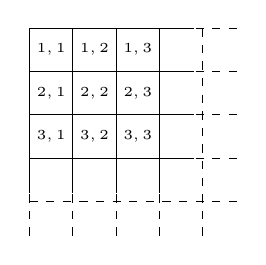
\begin{tikzpicture}[rotate=-90, scale=.55]
        \draw (1, 1) grid (4.8, 4.8);
        \draw[dashed] (1, 1) grid (5.8, 5.8);
        \foreach \i in {1, 2, 3} {
                \foreach \j in {1, 2, 3} {
                        \draw (\i, \j) rectangle (\i + 1, \j + 1) node[pos=.5] {\tiny \(\i, \j\)};
                    }
            }
    \end{tikzpicture}
    \caption{The set \(\positives^2\), with its elements graphically represented as unit boxes in the plane. The elements of the subset \(\interval{3}^2 \subset \positives^2\) are labeled with their coordinates.}
    \label{fig:positives2}
\end{figure}

The set \(\positives^2\) is partitioned into \vocab{rows}, where the \(i\)\textsuperscript{th} row is the set \(\{i\} \times \positives\),
and also partitioned into \vocab{columns}, where the \(j\)\textsuperscript{th} column is the set \(\positives \times \{j\}\).

\newcommand\coordleq{\leq_\mathrm{coord}}

The \vocab{coordinatewise partial order} on \(\positives^2\) is the partial order \(\coordleq\) given by
\begin{equation*}
    (i, j) \coordleq (i', j') \qquad \text{if and only if} \qquad i \leq i' \quad \text{and} \quad j \leq j'.
\end{equation*}
See Figure~\ref{fig:coordleq} for a graphical representation of the coordinatewise partial order \(\coordleq\) on \(\positives^2\).

\begin{figure}[htbp]
    \centering
    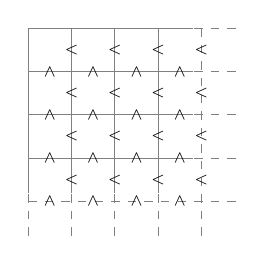
\begin{tikzpicture}[rotate=-90, scale=.55]
        \draw[black!50] (1, 1) grid (4.8, 4.8);
        \draw[black!50, dashed] (1, 1) grid (5.8, 5.8);
        \foreach \i in {1, 2, 3, 4} {
                \foreach \j in {1, 2, 3, 4} {
                        \node at (\i + .5, \j + 1) {\tiny \(<\)};
                    }
            }
        \foreach \i in {1, 2, 3, 4} {
                \foreach \j in {1, 2, 3, 4} {
                        \node[rotate=-90] at (\i + 1, \j + .5) {\tiny \(<\)};
                    }
            }
    \end{tikzpicture}
    \caption{The set \(\positives^2\), with its elements ordered by the coordinatewise partial order \(\coordleq\).
        Although only the relations between adjacent elements are shown, the relation between an arbitrary pair of elements is determined by the transitivity of the relations in the figure.}
    \label{fig:coordleq}
\end{figure}

A \vocab{Young diagram} is a diagram \(D \subset \positives^2\) such that, if \((i, j) \in D\), then \((i', j') \in D\) for all \((i', j') \coordleq (i, j)\).
Given a partition \(\lambda\), \vocab{the Young diagram of the partition} \(\lambda\) is the subset of \(\positives^2\) given by
\begin{equation*}
    \left\{ (i, j) \in \positives^2 \ : \  j \leq \lambda_i \right\}.
\end{equation*}
For example, the Young diagram of \(\composition{3, 3, 1}\) is the subset of \(\positives^2\) given by
\begin{equation*}
    \Big\{ (1, 1), (1, 2), (1, 3), \quad (2, 1), (2, 2), (2, 3), \quad (3, 1) \Big\},
\end{equation*}
which is graphically represented in Figure~\ref{fig:youngdiagram}.

\begin{figure}[htbp]
    \centering
    \ydiagram{3, 3, 1}
    \caption{The Young diagram of the partition \(\composition{3, 3, 1}\).}
    \label{fig:youngdiagram}
\end{figure}

As an abuse of notation, we use \(\lambda\) to denote both the partition and its Young diagram.

\section{Counting Vector Spaces}

\begin{definition}[Grassmanian]
    Let \(\mathbb{K}\) be a field,
    \(V\) be a vector space over \(\mathbb{K}\),
    and \(d \in \nonnegatives\).
    The \vocab{Grassmannian} \(\Grassmanian_d(V)\) is the set of all \(d\)-dimensional subspaces of \(V\).
\end{definition}

\begin{definition}
    The \vocab{\(q\)-binomial coefficient}, or \vocab{Gaussian coefficient}, is
    \[
        \qbinom{n}{k} = \prod_{i=0}^{k-1} \frac{1 - q^{n-i}}{1 - q^{k-i}}.
    \]
\end{definition}

\begin{proposition}[\(q\)-binomial coefficient recursion]
    For all \(n, k \in \positives\),
    \[
        \qbinom{n}{k} =
        \begin{cases}
            1 & \text{if } k = 0 \text{ or } k = n, \\    
            \qbinom{n-1}{k} + q^{n-k} \qbinom{n-1}{k-1} & \text{otherwise}.
        \end{cases}
    \]
\end{proposition}

\begin{corollary}
    The \(q\)-binomial coefficient is a polynomial in \(q\) with nonnegative integer coefficients.
\end{corollary}

\begin{corollary}
    For all \(n, k \in \positives\),
    \[
        \qbinom[1]{n}{k} = \binom{n}{k}.
    \]
\end{corollary}

\begin{lemma} \label{lem:grassmanian_qbinomial_prime_power}
    Let \(p\) be a prime, \(m \in \positives\), and \(\ell, w \in \nonnegatives\).
    Let \(q = p^m\).
    Then,
    \[
        \qbinom{\ell + w}{\ell}
        = \left|
            \Grassmanian_\ell\left(\finitefield{q}^{\ell + w} \right)
        \right|
        = \sum{\lambda \in \Par_{\ell, w}} (q)^{|\lambda|}.
    \]
\end{lemma}

\begin{proof}[Proof of the first equality.]
    Let \(\mathcal{M}\) be the set of all \(\ell \times (\ell + w)\) matrices with entries in \(\finitefield{q}\) with linearly independent rows.

    On one hand, we may count the elements of \(\mathcal{M}\) by choosing the \(\ell\) linearly independent rows one by one.
    There are \(q^{\ell + w} - 1\) choices for the first row,
    \(q^{\ell + w} - q\) choices for the second row, and so on.
    In general, there are \(q^{\ell + w} - q^{i-1}\) choices for the \(i\)\textsuperscript{th} row.
    Therefore,
    \begin{equation*}
        \left|
            \mathcal{M}
        \right|
        = \prod_{i=1}^{\ell} (q^{\ell + w} - q^{i-1})
    \end{equation*}

    On the other hand, we may count the elements of \(\mathcal{M}\) by first choosing the linear span of its rows, and then choosing the rows themselves in such linear span.
    There are \(|\Grassmanian_\ell(\finitefield{q}^{\ell + w})|\) choices for an \(\ell\)-dimensional subspace of \(\finitefield{q}^{\ell + w}\).
    Given such a subspace,
    there are \(q^{\ell} - 1\) choices for the first row,
    there are \(q^{\ell} - q\) choices for the second row, and so on.
    In general, there are \(q^{\ell} - q^{i-1}\) choices for the \(i\)\textsuperscript{th} row.
    Therefore,
    \begin{equation*}
        \left|
            \mathcal{M}
        \right|
        = \left|
            \Grassmanian_\ell\left(\finitefield{q}^{\ell + w} \right)
        \right|
        \prod_{i=1}^{\ell} (q^{\ell} - q^{i-1})
    \end{equation*}

    Finally, from the two expressions for \(\left| \mathcal{M} \right|\), we find
    \begin{align*}
        \left|
            \Grassmanian_\ell\left(\finitefield{q}^{\ell + w} \right)
        \right|
        = \prod_{i=1}^{\ell} \frac{q^{\ell + w} - q^{i-1}}{q^{\ell} - q^{i-1}} \\
        = \prod_{i=0}^{\ell - 1} \frac{1 - q^{\ell + w - i}}{1 - q^{\ell - i}} \\
        = \qbinom{\ell + w}{\ell},
    \end{align*}
    as desired for the first equality.
\end{proof}

\begin{proof}[Proof for the second equality]
    By linear algebra, the \(\Grassmanian_\ell(\finitefield{q}^{\ell + w})\) is in bijection with the set of \(\ell \times (\ell + w)\) matrices with independent rows and in row reduced echelon form.

    The set of \(\ell \times (\ell + w)\) matrices with independent rows and in row reduced echelon form is in bijection with the set of partitions of \(\ell\) with at most \(w\) parts by the following correspondence:
    \begin{quote}
        ``Start from the \(\ell \times (\ell + w)\) matrix with independent rows and in row reduced echelon form.
        There are \(\ell\) pivots, one in each row.
        Delete all zeroes southwest of the pivots, and delete all \(\ell\) pivot columns.
        The resulting matrix-looking table of elements of \(\finitefield{q}\) can be interpreted as an assignment of elements of \(\finitefield{q}\) to the boxes of the Young diagram within the rectangle of size \(\ell \times w\).''
    \end{quote}

    Note that, for each Young diagram within the rectangle of size \(\ell \times w\), there are \(q^{|\lambda|}\) ways to assign elements of \(\finitefield{q}\) to the boxes of the Young diagram.
    Therefore,
    \[
        \left|
            \Grassmanian_\ell\left(\finitefield{q}^{\ell + w} \right)
        \right|
        = \sum_{\lambda \in \Par_{\ell, w}} (q)^{|\lambda|},
    \]
    as desired for the second equality.
\end{proof}

\begin{theorem}
    Let \(\ell, w \in \nonnegatives\).
    Then,
    \[
        \sum_{\lambda \in \Par_{\ell, w}} q^{|\lambda|}
        = \qbinom{\ell + w}{\ell}.
    \]
\end{theorem}

\begin{proof}
    From Lemma~\ref{lem:grassmanian_qbinomial_prime_power},
    we know that the two polynomials agree at prime powers.
    Since the two polynomials agree at infinitely many points,
    they must be equal.
\end{proof}

\begin{definition}[Schubert cell]
    Let \(\lambda\) be a partition.
    Let \(V\) be a vector space of dimension \(d\), and let \(k\) be an integer such that \(0 \leq k \leq d\).
    The \vocab{Schubert cell} \(X^\circ_\lambda\) (of \(V\)) is the set of all \(k\)-dimensional subspaces of \(V\) such that \(\lambda\) is the Young diagram obtained from the unique \(k \times d\).
\end{definition}
    \chapter{Permutations}

Let \(n\) be a non-negative integer.
The \vocab{\(n\)\textsuperscript{th} symmetric group} \(\sym_n\)
is the group of bijections from \(\{1, 2, \ldots, n\}\) to itself,
under composition.
A permutation \(w \in \sym_n\) can be written in \vocab{two-line notation} as
\[
    \begin{pmatrix}
        1    & 2    & \cdots & n    \\
        w(1) & w(2) & \cdots & w(n)
    \end{pmatrix},
\]
or in \vocab{one-line notation} as
\[
    w(1)w(2)\cdots w(n).
\]
We may also think of a permutation \(w \in \sym_n\) as a directed graph with vertex set \(\{1, 2, \ldots, n\}\) and edges \(\{(i, w(i)) \mid i = 1, \ldots, n\}\). The connected components of this graph are cycles.


Each permutation \(w\) has an associated partition \(\cyc(w) \vdash n\) whose parts are the lengths of the cycles of \(w\), called the \vocab{cycle type} of \(w\). It is known that \(\cyc(w) = \cyc(u)\) if and only if \(w\) and \(u\) are conjugate in \(\sym_n\). Thus, the conjugacy class corresponding to a partition \(\lambda \vdash n\) is
\[
    \zeta_\lambda = \{ w \in \sym_n \mid \cyc(w) = \lambda \}.
\]

The centralizer of \(w \in \sym_n\) is
\[
    Z(w) = \{ u \in \sym_n \mid uw = wu \}.
\]
Let \(\lambda\) be a partition of \(n\), and let \(j_i\) be the number of parts of \(\lambda\) equal to \(i\). For \(w \in \zeta_\lambda\), the size of the centralizer is
\[
    |Z(w)| = \prod_{i=1}^n (j_i)! \prod_{k=1}^{\ell(\lambda)} \lambda_k,
\]
which does not depend on the choice of \(w \in \zeta_\lambda\). We denote this expression by \(z_\lambda\). Moreover, the size of the conjugacy class is
\[
    |\zeta_\lambda| = \frac{n!}{z_\lambda}.
\]

A permutation \(w \in \sym_n\) is called a \vocab{transposition} if \(\cyc(w) = 2\,1^{n-2}\), meaning \(w\) swaps two elements and fixes the rest. A \vocab{simple transposition} is a transposition of the form \(\eltr{i} = (i, i+1)\) for some \(i \in \{1, \ldots, n-1\}\).

The symmetric group \(\sym_n\) is generated by the simple transpositions \(\eltr{1}, \eltr{2}, \ldots, \eltr{n-1}\), subject to the relations:
\begin{align*}
    \eltr{i}^2                 & = 1,                                           \\
    \eltr{i}\eltr{j}           & = \eltr{j}\eltr{i} \quad \text{if } |i-j| > 1, \\
    \eltr{i}\eltr{i+1}\eltr{i} & = \eltr{i+1}\eltr{i}\eltr{i+1}.
\end{align*}
Groups with presentations similar to this one are called \vocab{Coxeter groups}.

Given a permutation \(w \in \sym_n\), an \vocab{inversion} is a pair \((i, j)\) such that \(i < j\) and \(w(i) > w(j)\). The number of inversions of \(w\) is denoted by \(\inv(w)\). The \vocab{Coxeter length} of \(w\) is the minimum number of simple transpositions needed to express \(w\) and equals \(\inv(w)\).

The \vocab{sign} of a permutation \(w\) is defined as \(\sign(w) = (-1)^{\inv(w)}\). This function \(\sign \colon \sym_n \to \{\pm 1\}\) is a group homomorphism. For \(w \in \zeta_\lambda\), we have \(\sign(w) = (-1)^{n - \ell(\lambda)}\), where \(\ell(\lambda)\) is the number of parts in \(\lambda\).

The symmetric group \(\sym_n\) has a unique element of minimum inversion number, namely the identity permutation \(\id\) with \(\inv(\id) = 0\), and a unique element of maximum inversion number, the permutation \(\omega_0 = n\, (n-1)\, \ldots\, 1\) with \(\inv(\omega_0) = \binom{n}{2}\).

For \(w \in \sym_n\), the \vocab{permutation matrix} \(M(w) \in \GL_n(\mathbb{C})\) is defined by \(M(w)_{ij} = \delta_{i, w(j)}\). The map \(M \colon \sym_n \to \GL_n(\mathbb{C})\) is a group homomorphism, and \(\sign\) equals the composition \(\det \circ M\).

A \vocab{(linear) representation} of a group \(G\) is a group homomorphism \(\rho \colon G \to \GL_n(\mathbb{C})\) for some \(n\). For example, \(M \colon \sym_n \to \GL_n(\mathbb{C})\) is a representation. A \vocab{permutation representation} of \(G\) is a homomorphism \(\rho \colon G \to \sym_n\) for some \(n\). Given any permutation representation \(\rho \colon G \to \sym_n\), composing with \(M\) yields a linear representation \(\rho' \colon G \to \GL_n(\mathbb{C})\).

Given a set \(S\) and a group action \(\rho \colon G \to \sym(S)\), the \vocab{fixed set} of \(S\) under \(\rho\) is
\[
    S^G = \{ s \in S \mid \rho(g)(s) = s \text{ for all } g \in G \}.
\]
Similarly, if \(V\) is a vector space with a representation \(\rho \colon G \to \GL(V)\), the \vocab{invariant subspace} is
\[
    V^G = \{ v \in V \mid \rho(g)v = v \text{ for all } g \in G \}.
\]
One can view \(V^G\) as the intersection of the eigenspaces associated with the eigenvalue \(1\) of the matrices \(\rho(g)\) for all \(g \in G\).

As an example, let \(\mathcal{G}_n\) be the set of all graphs on the vertex set \(\{1, 2, \ldots, n\}\). The group \(\sym_n\) acts on \(\mathcal{G}_n\) by permuting vertices: for \(w \in \sym_n\) and \(G \in \mathcal{G}_n\), the graph \(w \cdot G\) is obtained by applying \(w\) to the vertices of \(G\). Under this action, the only fixed graphs are the empty graph and the complete graph.

An \vocab{action of a group \(G\) on a ring \(R\)} is a group homomorphism \(\rho \colon G \to \Aut(R)\), where \(\Aut(R)\) is the group of ring automorphisms of \(R\). The fixed set \(R^G\) is a subring of \(R\).

An \vocab{algebra over a field \(k\)} is a vector space \(A\) over \(k\) equipped with a bilinear multiplication \(\cdot \colon A \times A \to A\). If \(A\) is a \(k\)-algebra, it contains a copy of \(k\) as a subring. Conversely, if \(A\) is a ring containing a field \(k\) as a subring, then \(A\) is a \(k\)-algebra.

Examples of \(k\)-algebras include the ring of polynomials \(k[x]\), the ring of power series \(k[[x]]\), and the ring of matrices \(\Mat_n(k)\).

Given \(k\)-algebras \(A\) and \(B\), a \vocab{\(k\)-algebra homomorphism} is a map \(\varphi \colon A \to B\) that is both a ring homomorphism and \(k\)-linear. An \vocab{action of a group \(G\) on a \(k\)-algebra \(A\)} is a group homomorphism \(\rho \colon G \to \Aut(A)\), where \(\Aut(A)\) is the group of \(k\)-algebra automorphisms of \(A\). The fixed set \(A^G\) is a \(k\)-subalgebra of \(A\).

A \vocab{monomial} is a product of powers of variables. In \(\mathbb{Q}[x_1, x_2, \ldots, x_n]\), monomials are indexed by \(\mathbb{N}^n\):
\[
    x^\alpha = x_1^{\alpha_1}x_2^{\alpha_2}\cdots x_n^{\alpha_n},
\]
for \(\alpha = (\alpha_1, \alpha_2, \ldots, \alpha_n) \in \mathbb{N}^n\). The \vocab{degree} of \(x^\alpha\) is \(\deg(x^\alpha) = \alpha_1 + \alpha_2 + \cdots + \alpha_n\). The set of monomials forms a basis for \(\mathbb{Q}[x_1, x_2, \ldots, x_n]\) as a vector space over \(\mathbb{Q}\).

We denote by \(\mathbb{Q}[x_1, x_2, \ldots, x_n]_d\) the subspace spanned by monomials of degree \(d\), giving the direct sum decomposition
\[
    \mathbb{Q}[x_1, x_2, \ldots, x_n] = \bigoplus_{d=0}^\infty \mathbb{Q}[x_1, x_2, \ldots, x_n]_d.
\]

The group \(\sym_n\) acts on monomials by
\[
    w \cdot x^\alpha = x^{w(\alpha)} = x_{w^{-1}(1)}^{\alpha_1}x_{w^{-1}(2)}^{\alpha_2}\cdots x_{w^{-1}(n)}^{\alpha_n}.
\]
This action extends linearly to \(\mathbb{Q}[x_1, x_2, \ldots, x_n]\). The \vocab{algebra of symmetric polynomials} is the subalgebra \(\Sym_n = \mathbb{Q}[x_1, x_2, \ldots, x_n]^{\sym_n}\) consisting of all polynomials fixed under this action.


    \printbibliography
\end{document}
